% !TEX root = ../main.tex

\section{The Derivative of Trigonometric Functions}
Looking at the graph of $y=\sin(x)$, Can we get an idea of how the derivative looks? \\
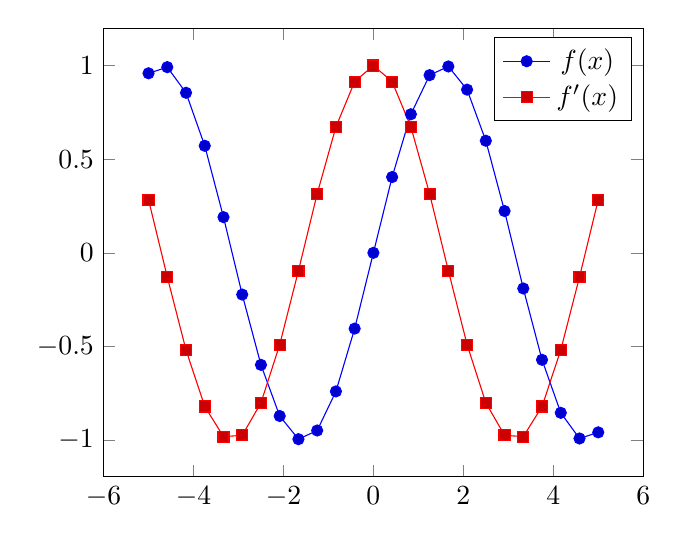
\begin{tikzpicture}
    \begin{axis}
        \addplot+ {sin(deg(x))};
        \addplot+ {cos(deg(x))};
        \legend{$f(x)$, $f'(x)$};
    \end{axis}
\end{tikzpicture}\\
The derivative of $y = \sin(x)$ is $y' = \cos(x)$
\subsection{Derivatives of $f(x) = \sin(x)$ and $f(x) = cos(x)$}
\begin{align}
    \deriv \left(\sin(x)\right) &= \cos(x) \\
    \deriv \left(\cos(x)\right) &= -\sin(x)
\end{align}
\begin{example}
    Find $\deriv \left(x\cos(x)\right)$
    \begin{align*}
        \deriv \left(x\right) &= 1 \\
        \deriv \left(\cos(x)\right) &= -\sin(x)
    \end{align*}
    \begin{gather*}
        x \cdot \deriv \left(\cos(x)\right) + \deriv \left(x\right) \cdot \cos(x) \\
        x \left(-\sin(x)\right) + 1 \cdot \cos(x) \\
        -x\sin(x) + \cos(x)
    \end{gather*}
\end{example}
\subsection{Derivative of $f(x) = \tan(x)$ }
\begin{equation}
    \deriv \left(\tan(x)\right) = \sec^2(x)
\end{equation}
\begin{proof}
    Proof that $\deriv\left(\tan(x)\right) = \sec^2(x)$.
    \begin{gather*}
        \deriv \left(\tan(x)\right) = \deriv \left(\dfrac{\sin(x)}{\cos(x)}\right) \\
        \dfrac{\cos(x) \cdot \cos(x) - \sin(x) \cdot - \sin(x)}{\cos^2(x)} \\
        \dfrac{\cos^2(x) + \sin^2(x)}{\cos^2(x)} \\
        \dfrac{1}{\cos^2(x)} \text{\quad -OR- \quad} 1 + \tan^2(x) \\
        \sec^2(x)
    \end{gather*}
\end{proof}
\begin{example}
    Find the derivative of $y = \cot(x)$ in two ways: Using $sin(x)$ and $cos(x)$, and using $tan(x)$. \\
    Method 1:
    \begin{gather*}
        \deriv\left(\dfrac{\cos(x)}{\sin(x)}\right) \\
        \dfrac{\sin(x) \cdot -\sin(x) - \cos(x) \cdot \cos(x)}{\sin^2(x)} \\
        \dfrac{-\sin^2(x) - \cos^2(x)}{\sin^2(x)} \\
        \dfrac{-\left(\sin^2(x) + \cos^2(x)\right)}{\sin^2(x)} \\
        -\dfrac{1}{sin^2(x)} \\
        -\csc^2(x)
    \end{gather*}
    Method 2:
    \begin{gather*}
        \deriv\left(\dfrac{1}{\tan(x)}\right) \\
        \dfrac{\tan(x) \cdot \deriv\left(1\right) - 1 \cdot \deriv\left(\tan(x)\right)}{\tan^2(x)} \\
        \dfrac{\cancel{\tan(x) \cdot 0} - \sec^2(x)}{\tan^2(x)} \\
        -\dfrac{\sec^2(x)}{\tan^2(x)} \\
        \dfrac{\dfrac{1}{\cancel{\cos^2(x)}}}{\dfrac{\sin^2(x)}{\cancel{\cos^2(x)}}} \\
        -\dfrac{1}{\sin^2(x)} \\
        -\csc^2(x)
    \end{gather*}
\end{example}
\subsection{Derivatives of SIX basic trig functions}
\begin{align}
    \deriv \left(\sin(x)\right) &= \cos(x) \\
    \deriv \left(\cos(x)\right) &= -\sin(x) \\
    \deriv \left(\tan(x)\right) &= \sec^2(x) \\
    \deriv \left(\cot(x)\right) &= -\csc^2(x) \\
    \deriv \left(\sec(x)\right) &= \sec(x)\tan(x) \\
    \deriv \left(\csc(x)\right) &= -\csc(x)\cot(x)
\end{align}
